\documentclass[10pt,a4paper]{article}
\usepackage[utf8]{inputenc}
\usepackage[english]{babel}
\usepackage{graphicx}
\usepackage{lmodern}
\usepackage{kpfonts}
\usepackage[left=2cm,right=2cm,top=2cm,bottom=2cm]{geometry}
\usepackage[export]{adjustbox}
\usepackage{dsfont}
\usepackage[noend]{algpseudocode}
\usepackage{wrapfig}
\usepackage{subcaption}
\usepackage{algorithm}
\newtheorem{lemma}{Lemma}
\newtheorem{definition}{Definition}
\newtheorem{notation}{Notation}
\newtheorem{proof}{Proof}
\author{Megi Dervishi}
\title{Algorithms and Programation}

\begin{document}

\maketitle
\section*{Homework 4 (5/01/2020)}
\subsection*{Exercise 1}
\subsection*{Solution}
\textbf{(1)}\\
We want to prove the following theorem: 
\begin{center}
$G$ \textit{is} $k$\textit{-edge-connected} $\Leftrightarrow$ $\forall (v_i,v_j), \, 1\leq i,j \leq n, \, i \neq j$ \textit{are joined by k-pairwise edge disjoint paths}
\end{center}
\textbf{Note:} There is an ambiguity on the term "path" on the theorem which actually intends "at least $k$ paths". For example the following graph is $2$-edge-connected but there are 3 disjoint paths between vertex 1 and 5.\begin{figure}[h!]
\centering
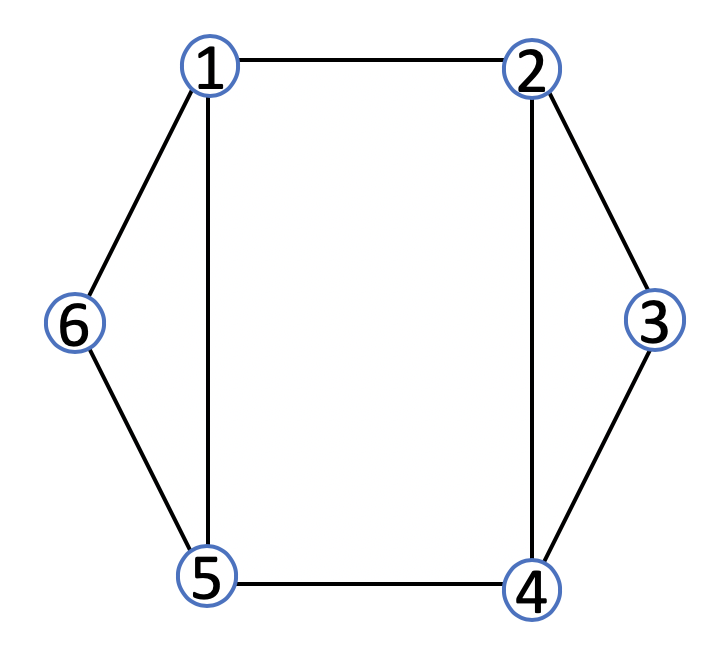
\includegraphics[width=0.15\textwidth]{graph}
\end{figure}
\\$\mathbf{(\Leftarrow)}$ Pair of vertices are joined by $k$-pairwise edge disjoint paths means that there are $k$-paths none of which share an edge between all pairs of vertices. So it is trivial to see that if you delete an edge from each $k$-paths i.e. $k$ edges, you have disconnected the graph. If you delete less than k-edge then since you have $k-$paths then there is at least $1$ path that is not destroyed so the graph would still be connected. Hence if every pair of vertices are joined by k pairwise edge disjoint paths then you need to delete at least $k$ edges to disconnect the graph i.e. $G$ is $k$- edge connected.\\\\
$\mathbf{(\Rightarrow)}$ For $G$ to be $k$-edge connected at least $k$ edges need to be cut in order to disconnect it. Let $X$ be the set of minimum edges which if removed they disconnect the graph into two parts $A$ and $B$. Consequently we have that $card(X) = k$. Let $\forall e \in G, \, c(e) = 1$. In other words "$G$ is $k$-edge connected" is equivalent to the minimum cut problem $\forall (s,t) \in A\times B$.  So the value of the minimum cut is $k$ since the minimum amount of edges you have to remove is $k$, ($card(X)$). By the max flow min cut theorem we have that the value of the minimum cut is equal to the value of the maximal flow i.e. $k$. Now we have two case:\\
\textbf{case 1:}  Fix $(s,t) \in A\times B$. We know that the maximal flow from $s$ to $t$ is $k$. Suppose that there were less than $k$ disjoint paths then the maximal flow would be strictly lower than $k$. So the value of maximal flow being $k$ forces that there must be $k$ disjoint paths. \\
\textbf{case 2:} Wlog, fix $(s,t) \in A$. Then either there exists another $X'$ such that the removal of it would separate the graph into a new $A', B'$ such that $s \in A'$ and $t \in B'$ or there exists no such set. If that's the case then by the contrapositive of the first implication proof we have that there are more than $k$ paths. Hence at least $k$ paths. 
In all cases there are at least $k$-pairwise edge disjoint paths $\forall s,t \in V$.\\\\By double implication this concludes the proof.\\\\
\textbf{(2)}
The algorithm takes as input an undirected graph $ G = (V, E)$ and outputs the minimum edge cut $X$. 
We start by replacing each undirected edge in $G$ with two oppositely directed edges both of capacity 1.  Let $G_f$ be the resulting graph. Then we choose an $s \in V$ at random and apply the Ford-Fulkerson algorithm $\forall t \in V\setminus \{s\}$ which will compute the maximum flow for all $t$. Then we take $t_{min}$ which has the minimal maximal flow and its residual graph $G_r$. By the corollary in the lecture we are sure that we can compute the min-edge-cut from $G_r$ (in linear time). The algorithm is correct and terminates. \\
\textbf{Time complexity} We are iterating over $n-1$ vertices the Ford-Fulkerson algorithm which has complexity $\mathcal{O}(fm) = \mathcal{O}(mn)$ since $f \leq nC = n$ and $C = 1$. Finally we compute the min-edge-cut in $\mathcal{O}(n)$ which makes the time complexity of our algorithm be $\mathcal{O}(mn^2)$. So our algorithm runs in poly-time. 


\subsection*{Exercise 2}
\subsection*{Solution}
First we show that the greedy algorithm terminates. Let $S_E$ be the set of edges of the cut which initially is equal to $\emptyset$. Let $|e_v|$ be the cardinality of incident edges of a vertex $v$. We know that $|e_v| = |nc_v| + |c_v|$ where $nc_v$ is the not-crossing edges and $c_v$ is the crossing edges of $v$. Also by step b we have that $|c_v| < \frac{1}{2}|e_v|$. Assume we want to add in the $S_E$ a new set of edges, call the new formed set $S'_E$. Hence we have that:
$$|S'_E| = |S_E|+|nc_v| -|c_v| = |S_E| +|e_v|-2|c_v| $$
$$ |S'_E| > |S_E| + |e_v| -2\frac{1}{2}|e_v| = |S_E| $$
So the cardinality is increasing and since $|S'_E|$ is bounded above by $|E|$ then that means that the algorithm terminates.\\
Now we show that the algorithm is a $2$-approximation of Max-Cut. Since this is a maximization problem then we need to prove that $ALG(P) \geq \rho(n) OPT(P)$ where $\rho(n) < 1$. Let $MC$ be the max-cut i.e. the optimal solution and $S_E$ the solution that the greedy algorithm outputs. We notice at step b that we add more than $\frac{1}{2}$ of the incident edges so in the end that would result in the following inequality $S_E \geq \frac{|E|}{2}$. Hence we have the following which proves that the greedy algorithm is 2-approximation of the Max-Cut:
$$|S_E| \geq \frac{1}{2}|E| \geq \frac{1}{2}|MC|$$
Finally we show that the randomized algorithm is also a $2$-approximation of the Max-Cut. We keep the same notation. Then using the linearity of expectation we have that:
\begin{align*}
\mathbb{E}[|S_E|] &= \sum_{(v_1,v_2) \in G.E} \mathbb{P}(v_1, v_2 \in A \times B \lor v_1, v_2 \in B \times A) = \sum_{(v_1, v_2) \in G.E} (\mathbb{P}(v_1,v_2 \in A \times B) + \mathbb{P}(v_1, v_2 \in B \times A))\\
&= \sum_{(v_1, v_2) \in G.E} (\frac{1}{4} + \frac{1}{4} ) = \frac{|E|}{2} \geq \frac{1}{2} |MC|
\end{align*}

\subsection*{Exercise 3}
\subsection*{Solution}
"Become infinitely rich" means that there exists a sequence of currencies $c_1, \cdots c_k$ that when multiplying their exchange rates, the product will be bigger than $1$ i.e. $$ R[i_1,i_2]\cdot R[i_2,i_3]\cdots R[i_{k-1},i_k]\cdot R[i_k,i_1] > 1 $$  We transform this sequence  in the following way so we could apply the Bellman-Ford algorithm which returns False if there exists a negative cycle in the weighted graph of currencies:
$$ \log (R[i_1,i_2]\cdot R[i_2,i_3]\cdots R[i_{k-1},i_k]\cdot R[i_k,i_1]) > \log(1) $$  
$$ \log(R[i_1,i_2]) + \log( R[i_2,i_3])+ \cdots \log( +R[i_{k-1},i_k]) +\log( R[i_k,i_1]) > 0 $$  
$$ -\log(R[i_1,i_2]) - \log( R[i_2,i_3])- \cdots \log( -R[i_{k-1},i_k]) -\log( R[i_k,i_1]) < 0 $$  
Hence if the algorithm returns False then there exists such a sequence in the graph, i.e. it is time to become rich.
The time complexity of the Bellman-Ford algorithm is $\mathcal{O}(VE)$. Assume we have $n$ vertices then in a complete digraph we would have $\frac {n^2-1} {2}$ edges so the time complexity is $\mathcal{O}(n^3)$. The printing and transforming of such sequence back to its original form would take $\mathcal{O}(n)$. In conclusion this algorithm would be of time complexity $\mathcal{O}(n^3)$ and space complexity $\mathcal{O}(n^2)$ (for the storing of the table $R$).


\end{document}